\documentclass[]{article}
\usepackage{lmodern}
\usepackage{amssymb,amsmath}
\usepackage{ifxetex,ifluatex}
\usepackage{fixltx2e} % provides \textsubscript
\ifnum 0\ifxetex 1\fi\ifluatex 1\fi=0 % if pdftex
  \usepackage[T1]{fontenc}
  \usepackage[utf8]{inputenc}
\else % if luatex or xelatex
  \ifxetex
    \usepackage{mathspec}
  \else
    \usepackage{fontspec}
  \fi
  \defaultfontfeatures{Ligatures=TeX,Scale=MatchLowercase}
\fi
% use upquote if available, for straight quotes in verbatim environments
\IfFileExists{upquote.sty}{\usepackage{upquote}}{}
% use microtype if available
\IfFileExists{microtype.sty}{%
\usepackage{microtype}
\UseMicrotypeSet[protrusion]{basicmath} % disable protrusion for tt fonts
}{}
\usepackage[margin=1in]{geometry}
\usepackage{hyperref}
\hypersetup{unicode=true,
            pdftitle={Analysis of electric vehicle usage patterns in New Zealand},
            pdfauthor={Rafferty Parker and Ben Anderson (University of Otago)},
            pdfborder={0 0 0},
            breaklinks=true}
\urlstyle{same}  % don't use monospace font for urls
\usepackage{longtable,booktabs}
\usepackage{graphicx,grffile}
\makeatletter
\def\maxwidth{\ifdim\Gin@nat@width>\linewidth\linewidth\else\Gin@nat@width\fi}
\def\maxheight{\ifdim\Gin@nat@height>\textheight\textheight\else\Gin@nat@height\fi}
\makeatother
% Scale images if necessary, so that they will not overflow the page
% margins by default, and it is still possible to overwrite the defaults
% using explicit options in \includegraphics[width, height, ...]{}
\setkeys{Gin}{width=\maxwidth,height=\maxheight,keepaspectratio}
\IfFileExists{parskip.sty}{%
\usepackage{parskip}
}{% else
\setlength{\parindent}{0pt}
\setlength{\parskip}{6pt plus 2pt minus 1pt}
}
\setlength{\emergencystretch}{3em}  % prevent overfull lines
\providecommand{\tightlist}{%
  \setlength{\itemsep}{0pt}\setlength{\parskip}{0pt}}
\setcounter{secnumdepth}{5}
% Redefines (sub)paragraphs to behave more like sections
\ifx\paragraph\undefined\else
\let\oldparagraph\paragraph
\renewcommand{\paragraph}[1]{\oldparagraph{#1}\mbox{}}
\fi
\ifx\subparagraph\undefined\else
\let\oldsubparagraph\subparagraph
\renewcommand{\subparagraph}[1]{\oldsubparagraph{#1}\mbox{}}
\fi

%%% Use protect on footnotes to avoid problems with footnotes in titles
\let\rmarkdownfootnote\footnote%
\def\footnote{\protect\rmarkdownfootnote}

%%% Change title format to be more compact
\usepackage{titling}

% Create subtitle command for use in maketitle
\newcommand{\subtitle}[1]{
  \posttitle{
    \begin{center}\large#1\end{center}
    }
}

\setlength{\droptitle}{-2em}

  \title{Analysis of electric vehicle usage patterns in New Zealand}
    \pretitle{\vspace{\droptitle}\centering\huge}
  \posttitle{\par}
  \subtitle{Statistical Report}
  \author{Rafferty Parker and Ben Anderson (University of Otago)}
    \preauthor{\centering\large\emph}
  \postauthor{\par}
      \predate{\centering\large\emph}
  \postdate{\par}
    \date{Last run at: 2019-03-26 13:01:32}

\usepackage{booktabs}
\usepackage{longtable}
\usepackage{array}
\usepackage{multirow}
\usepackage{wrapfig}
\usepackage{float}
\usepackage{colortbl}
\usepackage{pdflscape}
\usepackage{tabu}
\usepackage{threeparttable}
\usepackage{threeparttablex}
\usepackage[normalem]{ulem}
\usepackage{makecell}
\usepackage{xcolor}

\begin{document}
\maketitle

{
\setcounter{tocdepth}{2}
\tableofcontents
}
\section{Key Findings:}\label{keyFindings}

Based on a relatively small sample of 44 domestic electric vehicles
provided by our research partner and monitored over 8 months from April
2018 to January 2019. The recorder provided measurements at 1 minute
frequency of charging power and battery charge state.

\begin{itemize}
\tightlist
\item
  \emph{Power supplied}: The median power supplied during a standard
  charging event was 1.78 kW. The mean was slightly higher at 2.12 kW.
  Fast charging observations had a median of 30.84 kW (mean = 30.68kW);
\item
  \emph{Charging duration}:Charging durations tended to fall into one of
  two groups. Longer `standard' charges had a median duration of 0.06
  hours and a mean duration of 1.69 hours. High power ``fast'' charge
  events had a median duration of 12.47 minutes and a mean duration of
  13.87 minutes.
\item
  \emph{Time of day}: Standard charging events tended to begin around
  10pm, suggesting the drivers in our dataset utilise timers to take
  advantage of off-peak electricity. Fast charging events tended to
  begin at 11:30am on weekdays and 1pm during weekends.
\item
  \emph{State of charge}: Many drivers begin recharging with greater
  than 50\% charge still remaining in the battery.
\end{itemize}

In concurrence with the 2018 Concept Consulting
report{[}@ConceptConsulting2018{]}, these findings suggest that any
negative effects electric vehicles may have on the evening national
electricity grid peaks should be mitigable through ``smart'' charging
methods. In addition, our analysis indicates that this is already
occurring to some extent.

\section{Introduction}\label{introduction}

The New Zealand government has set a target of increasing the number of
electric vehicles (EVs) in New Zealand to 64,000 by
2021{[}@TranspowerNewZealand2017{]}. High penetration of EVs would cause
EV recharging to contribute a substantial portion of total electricity
load. A report prepared for lines companies Orion, Powerco and Unison by
Concept Consulting Group entitled ``Driving change - Issues and options
to maximise the opportunities from large-scale electric vehicle uptake
in New Zealand'' predicts that if all current light private vehicles
were electric, annual residential electricity consumption would increase
by approximately 30\%, whereas if all vehicles including trucks were
electric, this would increase the total electricity consumption of New
Zealand by approximately 41\%{[}@ConceptConsulting2018{]}.

New Zealand's total electricity demand varies throughout the day, with
weekdays in particular having two distinct ``peaks''; one in the
morning, and one in the evening{[}@TranspowerNZ2015{]}. Providing the
electricity to meet these demand peaks is a costly and inefficient
process{[}@Kahn2018{]}. Concurrent electric vehicle charging, especially
in the early evening when many motorists return home, would have the
potential to negatively impact the operation of the grid through
drastically increasing peak loads {[}@Azadfar2015{]}, leading to an
increased cost of electricity due to the requirement of expensive
upgrades to the electricity grid{[}@stephenson\_smart\_2017{]}.

The Concept Consulting report considers different methods of EV charging
in its models. The assumption that most drivers would begin charging
immediately after returning home is referred to as ``passive'' charging,
while charging that is programmed (either by the driver or by an
external entity) to occur during off-peak periods is referred to as
``smart''. The modelling undertaken in the Concept Consulting report
suggests that under a scenario whereby 57\% of the current private
vehicle fleet were EVs (corresponding to one EV per household), passive
charging would cause an increase of peak electricity demand of
approximately 3,000MW, whereas if all were charged in a ``smart''
fashion, there would be no increase in peak demand.

This report extends the work done by Concept Consulting, but utilises
actual data collected from electric vehicles, as opposed to using models
based on the current New Zealand transport sector. The intention of the
report is to provide further insight into the potential effects on the
New Zealand electricity grid that may occur with a dramatic increase in
EVs, so that these may be planned for and mitigated. It is also inspired
by the
\href{https://assets.publishing.service.gov.uk/government/uploads/system/uploads/attachment_data/file/764270/electric-chargepoint-analysis-2017-domestics.pdf}{UK
DoT statistical report 2018}{[}@Eyers2018{]}.

\section{Data information}\label{data}

\subsection{Background}\label{background}

The data used has been provided by ``Flip the Fleet'', a community
organisation that hopes to increase uptake of electric vehicles in New
Zealand. Flip the Fleet have been collecting data on electric vehicle
usage patterns, collected using Exact IOT Limited's
\href{https://flipthefleet.org/ev-black-box/}{blackbox recorder}, a
small electronic device that connects to the vehicle's internal computer
and sends detailed data about the battery health, consumption, speed,
etc.

The data provided was collected from 50 individual vehicles over 8
months (April 2018 - January 2019). The recorder provided measurements
at 1 minute frequency of charging power and battery charge state. It is
important to note that these vehicles are driven by ``early adopters''
who have opted to collect their vehicle usage data, and therefore the
data may not be a precise representation of the usage patterns of
current or future EV drivers.

Due to privacy considerations, the data is not publicly available.

\subsection{Initial cleaning}\label{initial-cleaning}

There were 6 vehicles in the data provided that had no recorded charging
occur. These were immediately discarded leaving 44 remaining vehicles,
in total consisting of 1291881 data points.

Some instances of charging power greater than 120kW were recorded. These
were considered anomalies and discarded, as these exceed the capacity of
the highest charging stations available in New
Zealand{[}@ConceptConsulting2018{]}.

Instances of battery state of charge being greater than 100\% or less
than 0\% were also discarded.

\subsection{Definitions and preparation}\label{cleaning}

Charging data has been broadly separated into two separate categories,
``standard'' and ``fast''. Standard charging is defined to be when the
charger is reading less than 7kW - this is considered the upper limit of
what can be obtained from an ordinary home charging scenario without an
expensive wiring upgrade{[}@ConceptConsulting2018{]}. Fast charging is
all charging above 7kW, and would likely occur at designated and
purpose-built public charging stations.

The data was also categorised according to whether it was a weekday or
not. This allows analysis to occur of differing charging patterns
between weekdays and weekends, allowing for further accuracy in
determining the effects of electric vehicles on grid peaks.

In order to determine charging durations, rows were initially flagged as
``charging begins'' if the charging power was greater than zero and the
previous and following row's charging power were (respectively) equal to
zero and greater than zero. Similarly, rows were flagged as ``charge
ends'' if the charging power was greater than zero and the previous and
following row's charging power were (respectively) greater than zero and
equal to zero.

Using this method we obtained 7376 instances of charge beginning, and
7385 instances of charge ending. The additional 9 instances of the
charge ending than there are of the charge beginning may be due to the
first instance of data collection occurring during mid-charge for some
vehicles.

The charge duration was then calculated as being the time duration
between each pair of ``charge begins'' and ``charge ends'' flags.

Figure \ref{fig:durationHist} shows the overall distribution of all
charging sequences. Clearly there are very small and a few very large
values for both charging types.

\begin{figure}
\centering
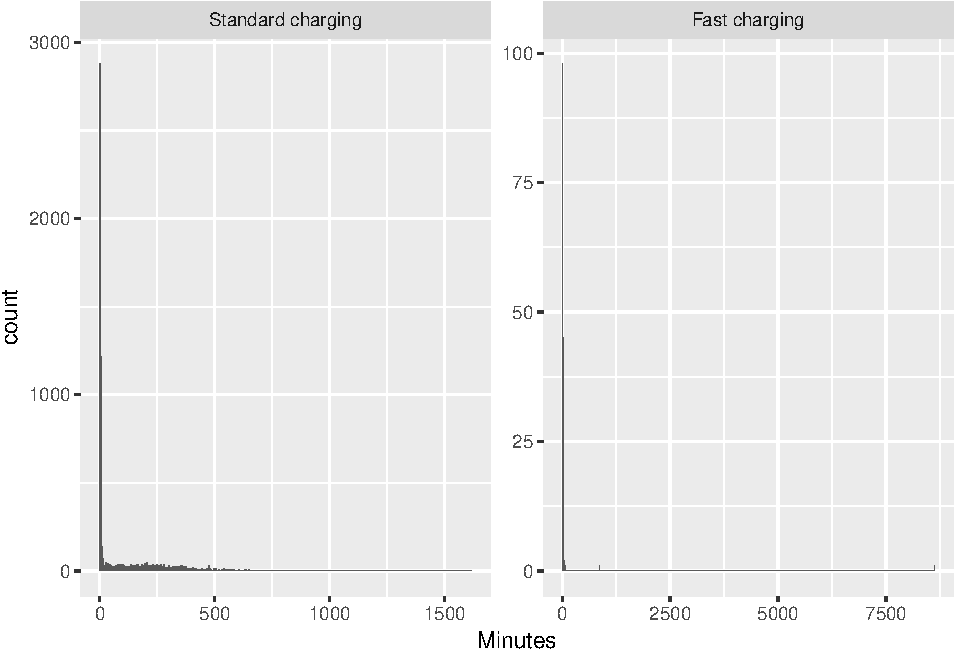
\includegraphics{EVBB_report_files/figure-latex/durationHist-1.pdf}
\caption{\label{fig:durationHist}Duration of charging sequences}
\end{figure}

Table \ref{tab:durationDescTable} shows the overall distributions and
indicates the extent to which the means are skewed by the very small and
a few very large values shown in Figure \ref{fig:durationHist}.

\begin{table}[t]

\caption{\label{tab:durationDescTable}Duration of all charge sequences by charge type (minutes)}
\centering
\begin{tabular}{l|r|r|r|r|r}
\hline
chargeType & N & mean & median & min & max\\
\hline
Standard charging & 6983 & 101.24 & 3.72 & 0.27 & 1616.72\\
\hline
Fast charging & 392 & 38.00 & 12.48 & 0.32 & 8621.00\\
\hline
\end{tabular}
\end{table}

Figure \ref{fig:shortDuration} shows the distribution of very short
charging sequences. As we can see these appear to be generally less than
8 minutes in length for Standard Charges.

\begin{figure}
\centering
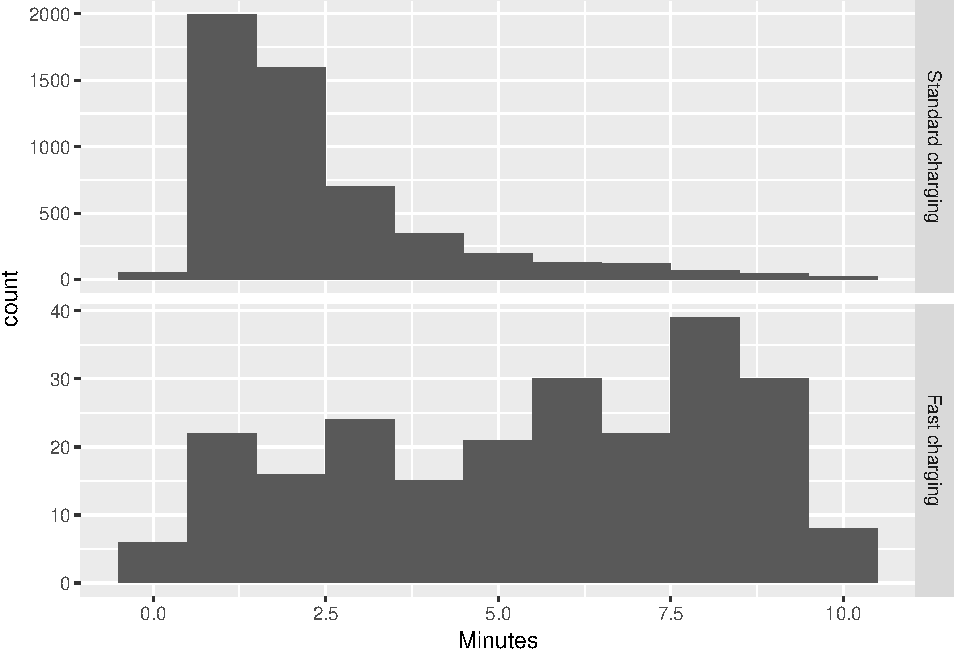
\includegraphics{EVBB_report_files/figure-latex/shortDuration-1.pdf}
\caption{\label{fig:shortDuration}Duration of charging sequences \textless{}
10 minutes}
\end{figure}

Table \ref{tab:durationDescTableReduced} shows the same descriptive
statistics but for all sequences of greater than 8 minute duration. Now
we can see that the mean and median durations for Standard Charge
sequences are closer to one another.

\begin{table}[t]

\caption{\label{tab:durationDescTableReduced}Duration of charge sequences > 8 minutes by charge type (minutes, )}
\centering
\begin{tabular}{l|r|r|r|r|r}
\hline
chargeType & N & mean & median & min & max\\
\hline
Standard charging & 2860 & 244.01 & 208.65 & 8.02 & 1616.72\\
\hline
Fast charging & 279 & 51.61 & 15.73 & 8.05 & 8621.00\\
\hline
\end{tabular}
\end{table}

Manual inspection of the data showed that these short-duration charging
``events'' generally occurred near the end of a longer-duration charging
event. It appeared that once the vehicle had reached its highest state
of charge, charging would intermittently stop and start again. This is
likely due to the behaviour of the charger once the battery was almost
full. In addition to the myriad ``short'' charging duration values, a
small amount of unreasonably long charging durations (longer than 100
hours for standard charging or longer than 14 hours for fast charging)
were calculated. As these exceeded the expected charge durations of the
most high capacity vehicles currently available, they were also assumed
to be anomalies. The analyses in Sections \ref{keyFindings} and
\ref{duration} were therefore made with these unreasonably long or short
duration charge events excluded from the data.

Figure \ref{fig:longDuration} shows the distribution of charging
sequences with the excessively long or short events removed. These
charging durations appear more reasonable when considering standard
battery capacities and charging powers.

\begin{figure}
\centering
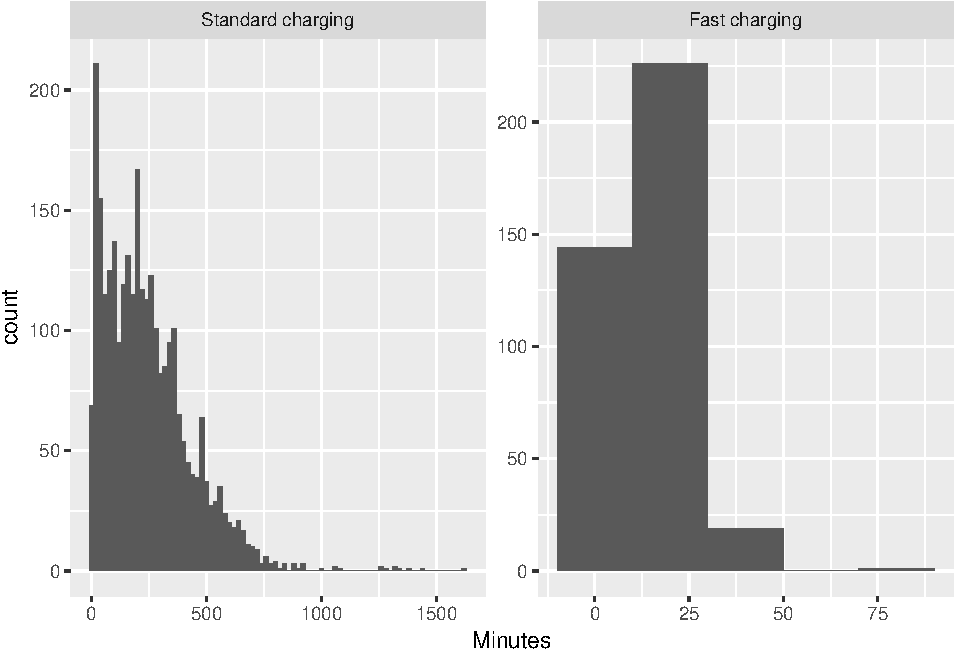
\includegraphics{EVBB_report_files/figure-latex/longDuration-1.pdf}
\caption{\label{fig:longDuration}Duration of charging sequences with
unreasonably long or short values removed}
\end{figure}

\begin{verbatim}
## Saving 6.5 x 4.5 in image
\end{verbatim}

\section{Observed demand}\label{observed-demand}

Figure \ref{fig:obsPower} shows the distribution of observed charging kW
demand by inferred charge type. This plot shows that fast charges are
relatively rare in the dataset whilst standard charges are much more
common, and are mostly concentrated around 1.8kW and 3kW, with a smaller
concentration around 6kW.

\begin{verbatim}
## `stat_bin()` using `bins = 30`. Pick better value with `binwidth`.
\end{verbatim}

\begin{figure}
\centering
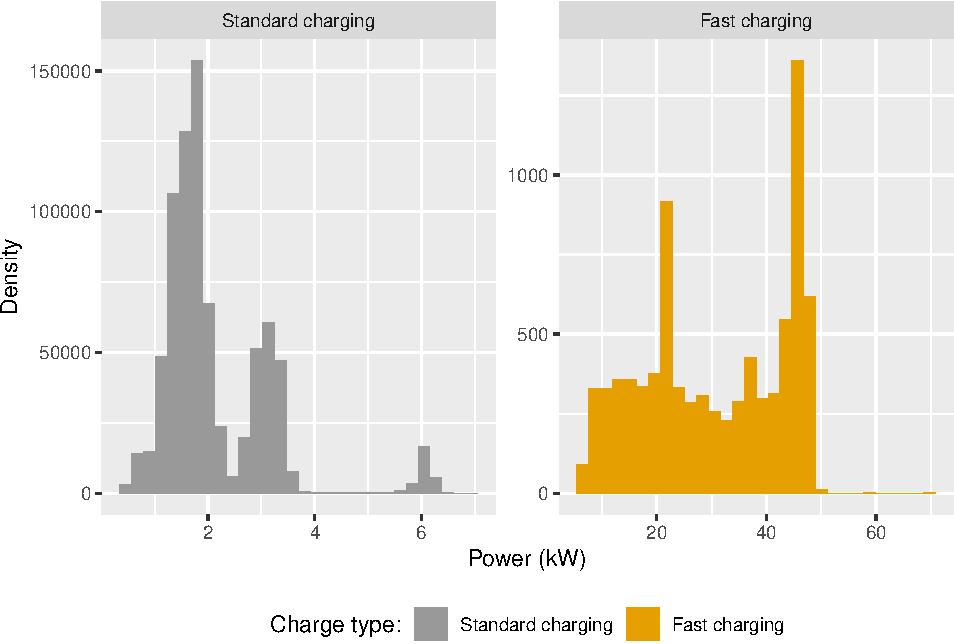
\includegraphics{EVBB_report_files/figure-latex/obsPower-1.pdf}
\caption{\label{fig:obsPower}Observed power demand distribution by charge
type where charging observed}
\end{figure}

75\% of standard charging observations were 1.47 kW or more but the
figure was 20.28 kW or more for fast charging

\section{Charging duration}\label{duration}

Figure \ref{fig:durationTimeMean} show that the duration of standard
charging events by event end time drops significantly for events ending
around 9:45am. This may indicate that people are plugging in after
returning home from a school run or other morning activity, even though
the battery is still close to full capacity. It may also suggest that
those who plug in shortly after 9:45am but do not have a high battery
state of charge are only ``topping up'', and take the vehicle out again
before charging is fully complete. Duration of fast charge events by
event end time appear to be more randomly distributed, although very few
events were recorded between midnight and 7am. This, along with the
comparatively low number of recorded fast charge events indicated in
Fig. \ref{fig:obsPower} suggests that drivers utilize fast charging only
``as necessary'' to ensure they have enough battery capacity to complete
their journey.

\begin{figure}
\centering
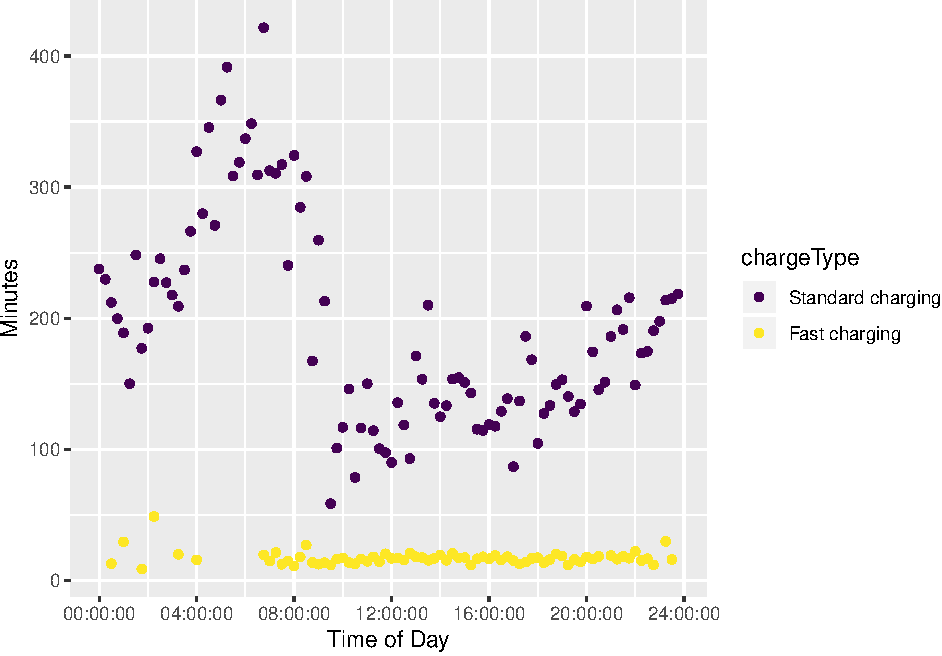
\includegraphics{EVBB_report_files/figure-latex/durationTimeMean-1.pdf}
\caption{\label{fig:durationTimeMean}Mean duration (within quarter hours) by
time of charging end}
\end{figure}

\begin{table}[t]

\caption{\label{tab:meanDurationTable}Mean duration of charge events by charge type}
\centering
\begin{tabular}{l|r|r|r|r|r}
\hline
chargeType & N & mean & median & min & max\\
\hline
Standard charging & 2860 & 244.00682 & 208.65000 & 8.016667 & 1616.717\\
\hline
Fast charging & 279 & 51.61231 & 15.73333 & 8.050000 & 8621.000\\
\hline
\end{tabular}
\end{table}

\section{State of charge}\label{SoC}

The state of charge is the percentage of energy still available to be
used in the battery. In future, electric vehicles may be able to
discharge any remaining battery charge as electricity into the grid, a
process known as vehicle to grid (V2G) energy transfer. This may allow
electric vehicles to have a net beneficial effect on the grid, reducing
the evening peaks by providing electricity to the home during this
period, and then recharging later in the evening or early the next
morning when peak demand has diminished.

This section provides an indication of the state of charge of electric
vehicles upon charging, so that the potential of V2G technology can be
assessed.

\begin{figure}
\centering
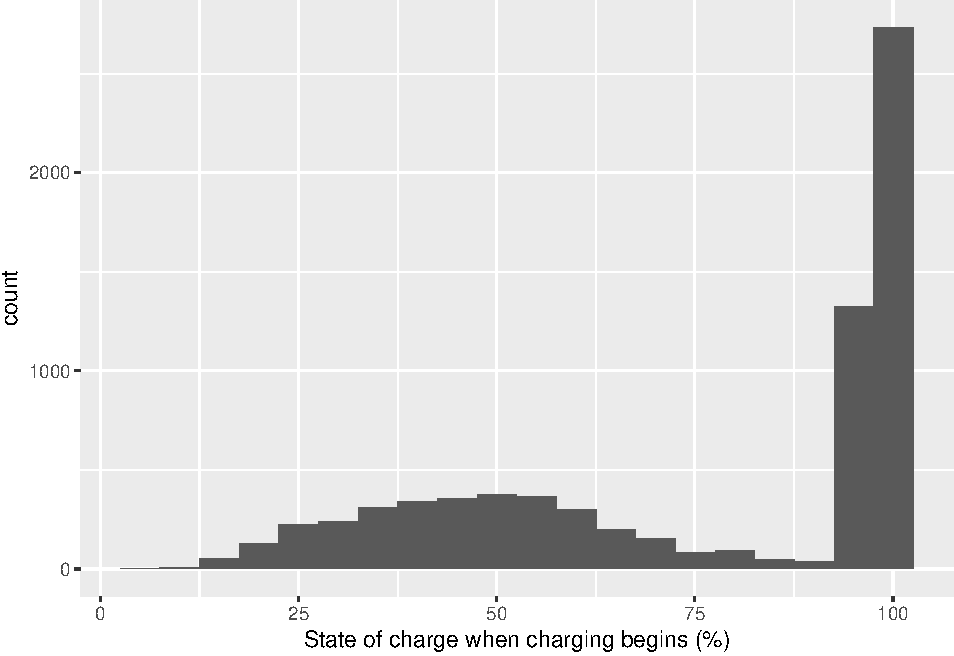
\includegraphics{EVBB_report_files/figure-latex/SoCplot1-1.pdf}
\caption{\label{fig:SoCplot1}Value of state of charge at beginning of
charge}
\end{figure}

\begin{verbatim}
## Saving 6.5 x 4.5 in image
\end{verbatim}

As can be seen in Figure \ref{fig:SoCplot1}, using the originally
defined ``charge begins'' data we have the majority of charges beginning
while the state of charge is above 90\%. This is likely due to the
manner in which the charger regularly turns off and on again near the
end of the charging cycle as described in Section \ref{cleaning}.

Figure \ref{fig:SoCplot2} shows the state of charge values when charge
begins but with state of charge greater than 90\% removed from the data
for clarity. The figure indicates that many vehicles begin charging
despite having greater than 50\% charge remaining.

\begin{figure}
\centering
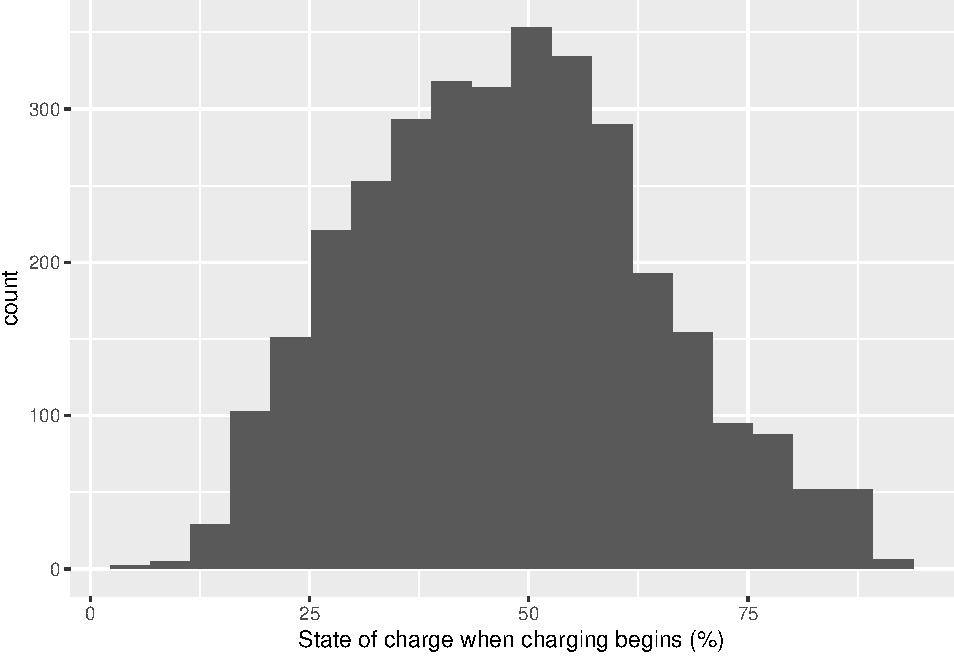
\includegraphics{EVBB_report_files/figure-latex/SoCplot2-1.pdf}
\caption{\label{fig:SoCplot2}Value of state of charge at beginning of charge
(\textgreater{}90\% values removed)}
\end{figure}

\begin{verbatim}
## Saving 6.5 x 4.5 in image
\end{verbatim}

\section{Time charging begins}\label{time-charging-begins}

After filtering out any data whereby charging begins while the state of
charge is greater than 90\% to account for battery `top-ups' (refer to
Section \ref{SoC}) we obtain the following figues.

\begin{verbatim}
## <ggproto object: Class FacetGrid, Facet, gg>
##     compute_layout: function
##     draw_back: function
##     draw_front: function
##     draw_labels: function
##     draw_panels: function
##     finish_data: function
##     init_scales: function
##     map_data: function
##     params: list
##     setup_data: function
##     setup_params: function
##     shrink: TRUE
##     train_scales: function
##     vars: function
##     super:  <ggproto object: Class FacetGrid, Facet, gg>
\end{verbatim}

\begin{figure}
\centering
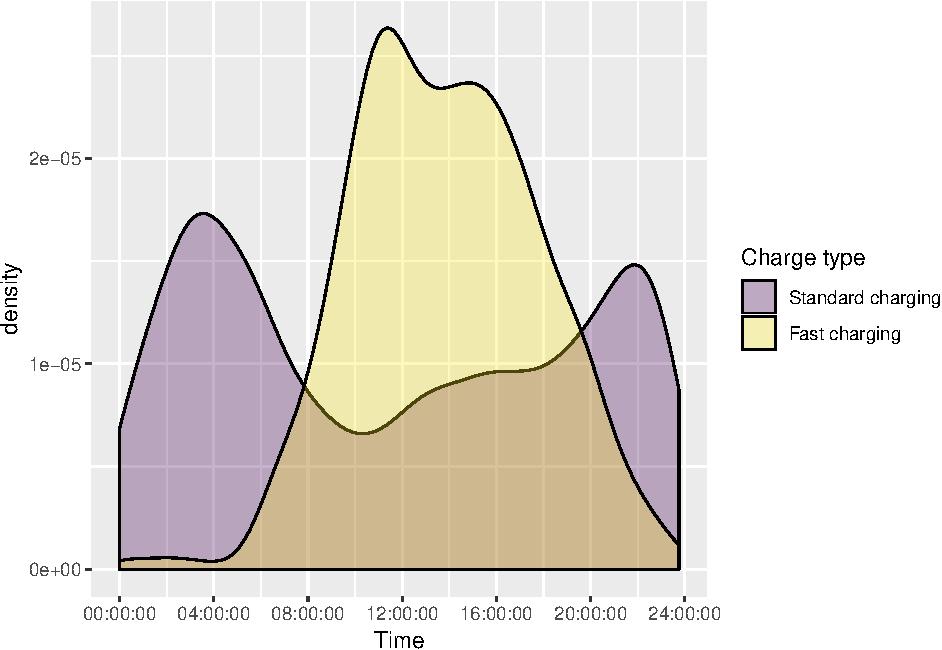
\includegraphics{EVBB_report_files/figure-latex/chargeBeginsWeekday-1.pdf}
\caption{\label{fig:chargeBeginsWeekday}Density plot of charging start times
during weekdays}
\end{figure}

\begin{verbatim}
## Saving 6.5 x 4.5 in image
\end{verbatim}

\begin{figure}
\centering
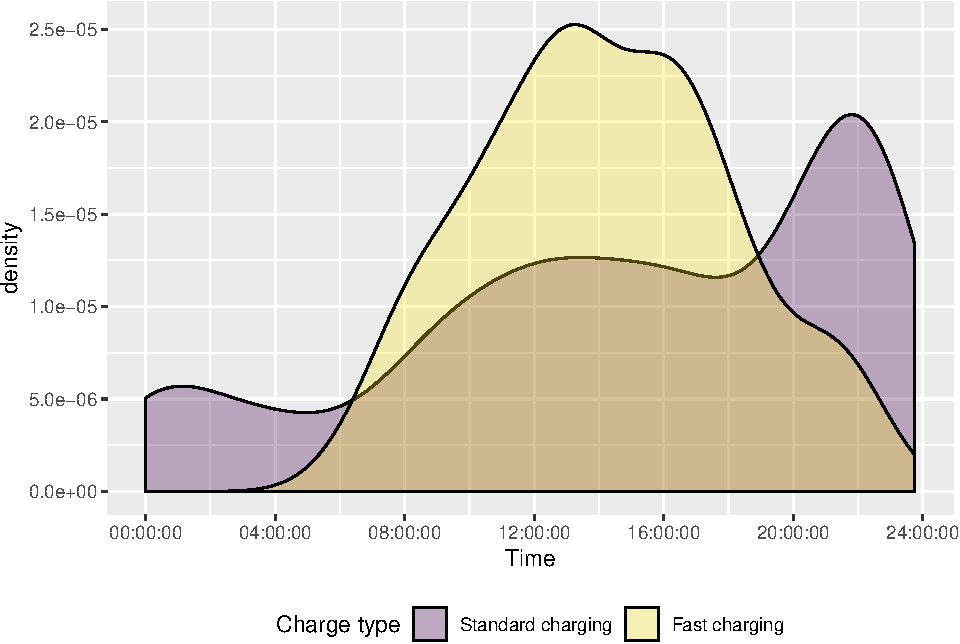
\includegraphics{EVBB_report_files/figure-latex/chargeBeginsWeekend-1.pdf}
\caption{\label{fig:chargeBeginsWeekend}Density plot of charging start times
during weekends}
\end{figure}

\begin{verbatim}
## Saving 6.5 x 4.5 in image
\end{verbatim}

Standard charging has a noticeably different profile to charging
patterns for fast charges. It suggests that it is common for plug-in
vehicle owners to charge overnight at home, and perhaps use the more
powerful public charge points to top up during the day.

Standard charging events most commonly began around 10pm during both
weekdays and weekends. As it seems unlikely that this is due to vehicle
drivers returning home at this hour, this effect may be due to drivers
setting the charger on a timer to take advantage of cheaper ``off-peak''
electricity times, which frequently begin around 10pm.

Fast charging events tended to begin at 11:30am on weekdays and 1pm
during weekends.

\begin{figure}
\centering
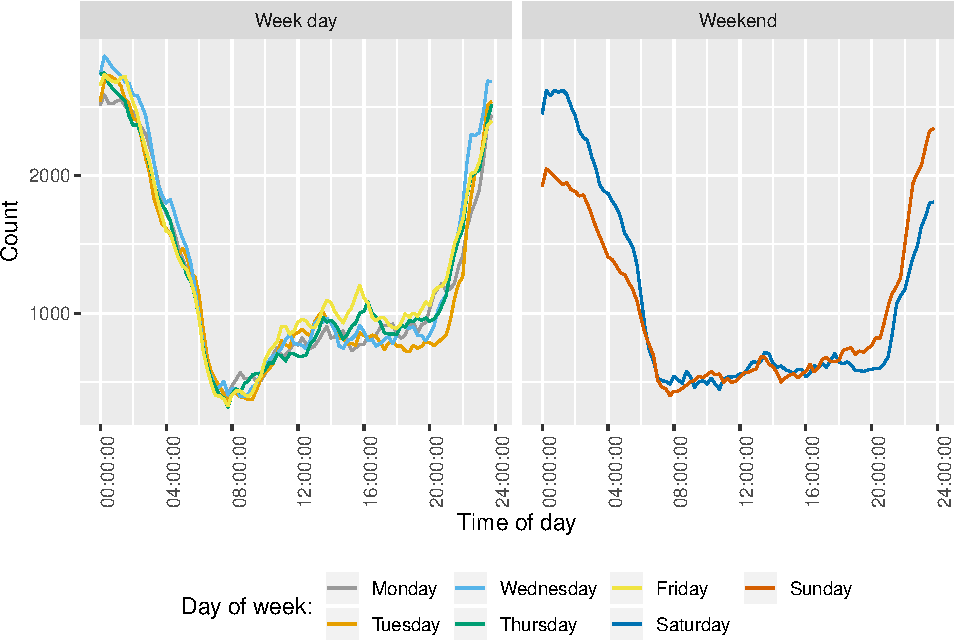
\includegraphics{EVBB_report_files/figure-latex/chargeTime-1.pdf}
\caption{\label{fig:chargeTime}Count of observed charging events by type,
day of week and time}
\end{figure}

Figure \ref{fig:chargeTime} shows the distribution of observed charging
by time of day and day of the week. This figure indicates greatest
charging occurance between the hours of 8pm and 8am, with very low
occurrences of charging during morning and evening grid peaks.

\section{Summary}\label{summary}

In the data provided for this study, most charging occurs at home using
either a 1.8kw or 3kW charger, and commonly occurs through the night as
opposed to during current grid peaks. In addition, many vehicles begin
charging with significant battery capacity remaining, providing them
with the ability to provide vehicle to grid energy transfer should that
technology become widely available.

If later adopters of electric vehicles can be induced to follow the same
``smart'' charging patterns as those displayed in our data sample, we
propose the effects that electric vehicles have on the electricity grid
may not be particularly negative.

\section{References}\label{references}


\end{document}
